\documentclass{article}[12pt]
\usepackage{hyperref}
\usepackage{indentfirst}
\usepackage{times}
\usepackage{amsmath}
\usepackage{amssymb}
\usepackage{csquotes}
\usepackage{graphicx}
\usepackage{subcaption}
\usepackage{listings}
\graphicspath{{./figures/}}



\title{A Case Against AI}
\author{Violet French}
\date{\today}


\begin{document}
\maketitle
\newpage
\tableofcontents
\listoffigures
\newpage

\section{Introduction}
With the recent advancements in Artificial Intelligence (AI) technology there arises a question of how and whether this technology should be used. Should Large Language Models (LLMs) be used in education? Is the use of AI moral? 

%%%%%%%%%%%%%%%%%%%%%%%%%%%%%%%%%%%%%%%%%%%%%%%%%%%%%%%%%% TODO: Change this Introduction %%%%%%%%%%%%%%%%%%%%%%%%%%%%%%%%%%%%%%%%%%%%%%%%%%%%%%%%%

\section{A Case Against AI in Education}
One of the places many argue AI is useful is in education. Many instructors today encourage students to use AI and some even use AI in grading and instruction. This section aims to discuss the costs of using AI in education and make a case against it's use in teaching the next generation.

\subsection{What is Memory}
Memory encompasses all the procedures by which our brains store and retrieve past information. When we experience some sensation, called a stimuli, our brains will process that information in a varity of ways. Most models of memory seperate memory into two distinct parts: Short Term Memory (STM) and Long Term Memory (LTM).\footnote{\raggedright Types of memory. Queensland Brain Institute - University of Queensland. (2024, September 25). https://qbi.uq.edu.au/memory/types-memory} STM stores things we only need for a short while, these memories could last few seconds up to a few minutes.\footnote{\raggedright What is short-term memory. Cleveland Clinic. (2025, October 2). https://my.clevelandclinic.org/health/articles/short-term-memory} LTM stores memories for a long period of time, this could be a few days or even the rest of our life. Long term memories always pass through short term memory first. In order to remember something for a long time it has to be remembered for a short time first. You've probably noticed this when learning something new. At first it feels as though you can never remember it but eventually it finds its place in your long term memory. There are many different models for memory which will not be discussed here but the reader may find them useful in understanding the processes by which we store things long term. The process of converting a stimuli or event into a memory is called encoding and gets its name from how computers encode information into memory.
\subsection{Rehearsal, Consolidation, and Reconsolidation}
\subsubsection{Consolidation}
Short term memory is naturally labile. Labile means that short term memory is subject to change very easily and it is considered unstable during this stage. This is great for learning as it makes first exposure to a topic to be most productive. Understanding on the topic can easily change and morph while it is in STM.

\begin{displayquote}

Systems consolidation is typically, and accurately, described as the process by which memories, initially dependent on the hippocampus, are reorganized as time passes. By this process, the hippocampus gradually becomes less important for storage and retrieval, and a more permanent memory develops in distributed regions of the neocortex. The idea is not that memory is literally transferred from the hippocampus to the neocortex, for information is encoded in the neocortex as well as in hippocampus at the time of learning. The idea is that gradual changes in the neocortex, beginning at the time of learning, establish stable long-term memory by increasing the complexity, distribution, and connectivity among multiple cortical regions.\footnote{\raggedright Squire, L. R., Genzel, L., Wixted, J. T., \& Morris, R. G. (2015). Memory consolidation. Cold Spring Harbor perspectives in biology, 7(8), a021766. https://doi.org/10.1101/cshperspect.a021766}

\end{displayquote}

This is similar (with some notable differences) to moving some item from volatile Random Access Memory (RAM) to a non-volatile Solid State Drive (SSD). With this analogy we should be aware that our memories are not actually moving unlike the data that goes between RAM and the SSD. Memory consolidation can be assisted through techniques like rehearsal. 

\subsubsection{Rehearsal}
Rehearsal is when we repeat exposure to a stimulus associated with that memory. The stimuli does not have to be the same as the one that a person was initially exposed to. For example, when learning a math topic one does not need to rewatch the lecture to study it, rather they can review notes or work through practice problems. These would be examples of generalizations of stimuli. While they are not identical to the original stimuli they are close enough that the brain will treat them in similar manners. In this case we are exposing ourselves to a similar context but different stimuli. We can also expose ourselves to a conditioned stimuli to rehearse. A conditioned stimuli is one which has been trained into someone through techniques of conditioning. Conditioning can be done in various ways, two well known examples are Ivan Pavlov's Classical Conditioning and B.F Skinner's Operant Conditioning. These techniques lead an individual to respond in a certain way to a conditioned stimuli. This is often used in training dogs to do tricks or to stop them from urinating on your carpet. These same techniques of conditioning work on humans.

\subsubsection{Reconsolidation}
When a memory arrives in long-term memory it becomes stable and isn't labile anymore, however long-term memories can become labile again. Long-term memories can become unstable on reactivation, such as when the memory is retrieved. This memory is then restabilized through reconsolidation. Going back to our computer memory example imagine we pulled new data into RAM from an SSD. When we have it in RAM it can easily be changed and updated. When we finally move this data back into the SSD (or stable LTM) this is reconsoldation. Some researchers will make a distinction between reconsolidation and updating long-term memories.

\subsection{Enhancing Memory Retention \& Formation}
\subsubsection{Rehearsal and Memory}
As discussed previously, memory consolidation is the stabilizing of short-term memories into long-term ones. This process can be aided in a variety of ways. One way we can aid the consolidation of memories is through simple rehearsal. A study on rats was done to test the effects of rehearsal on memory retention.\footnote{\raggedright Parle, M., Singh, N., \& Vasudevan, M. (2006). Regular rehearsal helps in consolidation of long term memory. Journal of sports science \& medicine, 5(1), 80–88.} Rats were subjected to various puzzles over four different testing periods. Groups were assigned to rats to determine how much they would be allowed to rehearse each puzzle. The results are outlined in Figure 1. This study demonstrates the importance of rehearsal in memory retention. Rats who rehearsed more performed better on puzzles even after several days had passed. 

% Figure 1 %
\begin{figure}[t!]
    \caption{Mice Rehearsal Memory Retention Results}

    \begin{subfigure}[H]{0.5\textwidth}
        \centering
        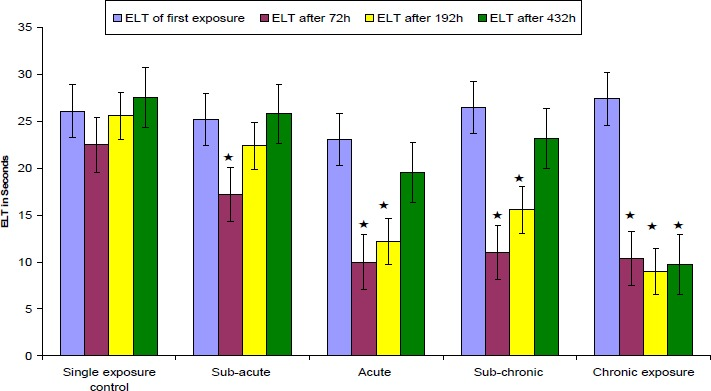
\includegraphics[scale=2]{RatMemoryPool.jpg}
        \caption{Escape Latency Time (ELT) of Rats in Hexagon Pool Swimming Puzzle}
    \end{subfigure}
    
    \begin{subfigure}[H]{0.5\textwidth}
        \centering
        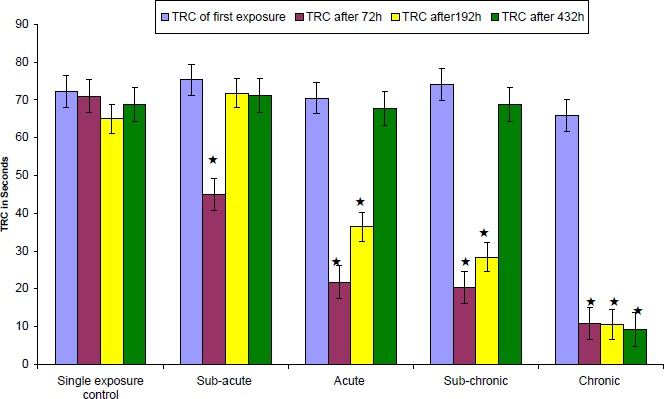
\includegraphics[scale=2]{RatMemoryRewardMaze.jpg}
        \caption{Time to Reach Reward Chamber (TRC) of Rats in Hebb-Williams Maze}
    \end{subfigure}

    \begin{subfigure}[H]{0.5\textwidth}
        \centering
        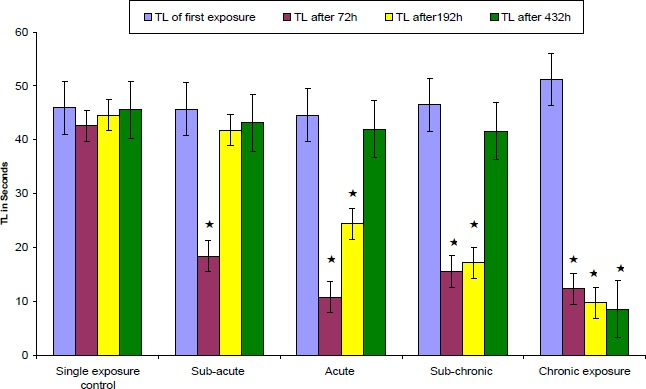
\includegraphics[scale=2]{RatsElevatedMaze.jpg}
        \caption{Time Latency (TL) of Rats in Elevated Maze}
    \end{subfigure}
\end{figure}

\subsubsection{Emotions}
Another way to improve memory consolidation is through a healthy amount of stress. Stress hormones modulate memory formation and retention.\footnote{\raggedright Bisaz, R., Travaglia, A., \& Alberini, C. M. (2014). The neurobiological bases of memory formation: from physiological conditions to psychopathology. Psychopathology, 47(6), 347–356. https://doi.org/10.1159/000363702} While too much stress is unhealthy and can impair memory a small amount of stress can aid in learning. Stress follows an inverse U shape with memory retention wherein small amounts and large amounts of stress are detrimental but a balance of the two is ideal for memory retention. When people experience too little stress they tend to consider it unimportant and when they experience too much stress they shut down, both prevent an individual from forming new memories or learning. Stress isn't the only emotion that affects memory formation, pleasurable emotions also increase memory retention and formation. Emotionally neutral experiences are quickly forgotten as opposed to ones with high levels of emotion. 

\subsubsection{Productive Struggle}
A term used in pedagogy is productive struggle. Productive struggle is a teaching technique often employed in math or programming courses but the ideas of it are prevalent to any topic one is learning. Productive struggle is when you allow students to struggle with the problem, limiting how much you help them. Rather than giving students the answer to the question immediately you allow them to work with the problem. This teaches students how to solve problems instead of just following procedure teaching them to confront problems in their own way. Productive struggle increases the production of myelin which helps with memory retention.\footnote{\raggedright What is productive struggle?. University of San Diego - Professional \& Continuing Education. (2026, August 18). https://pce.sandiego.edu/productive-struggle-in-the-classroom/ } Not immediately helping students allows them to struggle a bit, aiding in the process of developing memories. This does not mean students shouldn't get any help as this can be worse for the students. Instructors are encouraged to provide a safe environment to allow for questions to be asked and mistakes to be made. 

\subsubsection{Forgetting \& Retrieval}
Forgetting things and recalling them can be highly beneficial in aiding in memory retention. According to Bjork's Theory of Disuse\footnote{\raggedright Bjork, A., \& Bjork,. E. L. (1992). A new theory of disuse and an old theory of stimulus fluctuation. In A. Healy, S. Kosslyn, \& R. Shiffrin (Eds.), From Learning Processes to Cognitive "Processes: Essays in Honor of William K. Estes (Vol. 2, pp. 35-67). Hillsdale, NJ: Erlbaum. } our memories can be divided into two strength: storage and retrieval. Storage strength is how well learned that item is, or in other words, how much we know about it. Retrieval strength is how easily we can retrieve that item from memory. Retrieval strength slows the growth of storage strength. Lets think about a program, say we have massive data redundancy such that we have repeats of our data everywhere. This makes our data very accessible but trying to modify that data becomes painstaking as we need to change it in so many different locations. Often times these two strengths will grow together so this isn't much of a concern until you start to become an expert in a topic. When you know a lot about something it can become very hard to learn more about it. Storage strength never reduces, it is a misconception that memories decay with time. Instead memories become less accessible over time, with this understanding we can say retrieval strength may reduce over time. Retrieval strength can sometimes be lost when retrieval strength grows somewhere else. This is beneficial for humans since associating too many memories with one stimulus can make retrieval take longer as more filtering needs to be done. Imagine if every time someone asked you your location yesterday you had to figure out where you were out of all the possible places you have ever been. Instead our brains might only remember where we've been in the past week reducing how long it takes to recall the correct info. 

Some may think that studying is the best way to build memory retention but this is not true. While studying and learning more about a topic builds memory retention, recall builds retention far more. According to Bjork's theory, retrieval strength is built most by the simple act of recalling information from memory (remembering). The harder it is to remember, the more it builds retrieval strength. Retrieving things from memory also creates new associations with stimuli. If you associate more stimuli with a particular memory it becomes easier to access. You can think of stimuli like pointers in a programming language. Each pointer provides a way to access the same data. These pointers can also fall out of scope meaning they are no longer able to point to the same data, in other words the stimuli is no longer correlated with that memory. This lends credence to the idea that studying over multiple periods is more beneficial than cramming since studying multiple times means you need to do several retrievals for each study session rather than one retrieval for a cramming session. 

\subsubsection{Interleaving}
Interleaving is when one spreads out concepts of similar characteristics to aid in discrimination between topics. Some topics may use similar terms or have similar looking problems which can lead to students having difficulty figuring out what the answer to a problem is. Many textbooks teach in a block-based manner where similar information is grouped together in a way that can make it difficult for a student to differentiate between. Interleaving can solve this problem by spreading out similar information to aid in discriminating between topics.\footnote{\raggedright Rohrer, D., \& Hartwig, M. K. (2020). Unanswered questions about spaced interleaved mathematics practice. Journal of Applied Research in Memory and Cognition, 9(4), 433–438. https://doi.org/10.1016/j.jarmac.2020.06.008}

\subsection{AI Hurts Learning}
\subsubsection{Shortcutting the Difficulty}
As discussed earlier, difficulty is essential in the learning process. A common argument for AI in learning is that it makes learning easier. I believe this is the issue at hand. Learning is not supposed to be easy, it's supposed to challenge you to aid in the formation of new memories. We discussed earlier concepts such as productive struggle and the benefits of stress in learning. AI provides an easy out on the learning process by providing students with the answers depriving them of the important critical thinking skills they would have gained along the way. When one is simply given the answer to their question it becomes a mundane experience which is often promptly fogotten. When someone spends a significant amount of time challenging themselves to learn something and finally understands it, that experience sticks with them for a much longer time. Working through a problem by oneself also provides an unintended rehearsal session where they have to continue to look back at old information to try to decipher the new information. This helps provide more connections to the old information strengethening the students knowledge on the topic as a whole.

Another issue is one of self control. AI is more than capable of providing an answer to most questions one might have. When people feel challenged, such as when they don't immediately understand something, they feel a need to back away from the problem and try to find the easiest solution. In this way the relationship between a student and AI becomes one of dependence. Even the most capable students may find themselves retreating to AI when they are made uncomfortable. This leaves a student ill prepared for novel challenges they will inevitably face at some point in their lives. What happens when the AI cannot solve the problem, how will students combat this? These students have not had to be challenged, they haven't developed their problem solving skills. Learning is itself, a skill. Learning needs practice and when students shortcut the process they never learn how to learn.

\subsubsection{Missed Opportunities}
Another issue is one of missed opportunities. Often times we learn more than we originally intended to. Learning one thing often leads to the learning of many other things. These new concepts we learn along the way may provide us with the skills to combat other issues or motivate further research on related ideas. Falling into a rabbit-hole provides a great opportunity to answer questions you never thought you may have had. Being spoon-fed the answer by an AI model stops this opportunity for self-enrichment. Instead of learning all the little things that go into something you get a vapid answer from a prediction algorithm. Often these answer lack the nuance to be useful to the student in future endeavors. 

A great way to understand all this is to look at mathematics. A great misconception many have when it comes to math is the idea that mathematics is all about solving problems. While math spends a considerable amount of time teaching the student how to solve problems the real goal is to teach students how to understand problems. Knowing the answer without having an understanding of the process and applications is akin to a monkey with a typewriter, it will bear no fruit. As of writing this AI companies have launched hundereds of papers of mathematical proofs that were generated by LLMs. Terrence Tao, a respected mathemetician who worked on the Navier Stokes equation before it was allegedly solved by OpenAI, has often compared these AI proofs to strip mining.\footnote{https://mathstodon.xyz/@tao/117237320796901560}\footnote{https://www.numberphile.com/podcast/terence-tao-ai} I believe this strip mining occurs beyond the discipline of mathematics and is affecting students today. Students are robbed of future opportunities to learn by the very tools they think assist them in growing.


\begin{displayquote}
Nonetheless, while LLMs might in general be a more efficient way to acquire declarative knowledge, or knowledge on specific facts, our findings suggest that they may not be the best tool for developing deep procedural knowledge about a topic—that is, an understanding of how things work, and an ability to create new knowledge.\footnote{Shiri Melumad, Jin Ho Yun, Experimental evidence of the effects of large language models versus web search on depth of learning, PNAS Nexus, Volume 4, Issue 10, October 2025, pgaf316, https://doi.org/10.1093/pnasnexus/pgaf316}
\end{displayquote}

\subsubsection{High School Math Study}
A study was published back in October of 2025 that tested the effects of AI in teaching mathematics to high school students.\footnote{H. Bastani, O. Bastani, A. Sungu, H. Ge, Ö. Kabakcı, \& R. Mariman, Generative AI without guardrails can harm learning: Evidence from high school mathematics, Proc. Natl. Acad. Sci. U.S.A. 122 (26) e2422633122, https://doi.org/10.1073/pnas.2422633122 (2025).} To briefly summarize the paper, high school students were slated to be taught a new math concept. The researchers split students into three groups: GPT-Base, GPT-Tutor, and Control. The GPT-Base group were given Chat-GPT to use in studying and completing homework. The GPT-Tutor group were also given Chat-GPT but this version was specially prompted to act like a tutor and was given answers to the homework questions. Finally the control group was not permitted to use AI at all. The study performed two assessments: assignments and test. Assignments were administered to all groups and the number of correct answers were counted. For the assignments, students were permitted to use their AI to assist them in completion. For the test students were not allowed to use any AI and were reliant on their own knowledge. 

The GPT-Base group performed far worse on both the practice assignments and the final test. Researchers speculate students may have performed worse on the assignments because the AI was hallucinating and giving the wrong answers. This may have later led to students not knowing the concepts correctly by the time they reached the test

The GPT-Tutor group and Base group both performed similarly on tests with no statistically significant difference found. It appears that the tutor AI made no difference in the final results of the test. However the GPT-Tutor group did perform better on the practice assignments. This is speculated to be because students could have their work checked by the GPT-Tutor since the GPT-Tutor was given the answers to all the questions. This meant students could just get the answers without risks of hallucinations.

This study touches up upon another argument made by supporters of AI in education: If it's used correctly then it can be a useful tool. As we can see from this study, the specially prompted AI made no difference in the final knowledge assessment. So when used appropriately AI provides no tangible benefit and when used improperly the effects are very detrimental. High risk, no reward.

\subsection{Final Remarks}
With this section we asssessed a case against AI in education. While I believe many may not be convinced by moral arguments against AI I hope a practical argument like this has you reconsidering where you use AI. I implore you to consider the morality of AI as we discuss it in the next section and consider if using AI is an moral act.

\section{A Moral Argument Against AI}
In the competetive landscape of the world people often abandon their principles just to get ahead. Companies will damage the environment just to save a little bit of money or time. A common reason I've heard people justify their use of AI is that they don't want to fall behind. Many fear if they do not conform that they will be left behind. A question many of us must consider is whether we will stick to our principles when they are challenged. Do we give up on doing what we think is right because life has made it difficult to continue doing so? This is the question I would like you, the reader, to ponder as you read this section. What are your principles worth to you?
\subsection{Environmental Concerns}
\subsubsection{The Cost}
It is well known that AI server farms are highly detrimental for the environment. AI models rely heavily on arithmetic done on matrices which is highly unoptimized. Asymptotic analysis involves analyzing the efficiency of an algorithm by looking at how the complexity of an algorithm grows in proportion to its inputs. Many programmers are introduced to the idea of Big O notation for analyzing their algorithms. Big O notation is defined below

\[f(x) = O(g(x)) \iff \exists M : M \in \mathbb{R} \land M > 0 \land |f(x)| \le M \cdot g(x) ~ \forall x \in D\]

What this means is that some function $f(x)$ is said to be Big-O $g(x)$ if and only if there exists some value $M$ such that 
\begin{itemize}
\item $M$ is a real number
\item $M$ is greater than zero (positive)
\item The absolute value of $f(x)$ is less than or equal to $M \cdot g(x)$ for all x in D where D is the domain (all valid x values) of the function $f(x)$ 
\end{itemize}

In other words there is some value $M$ we can multiply $g$ by so that every value $x$ that we plug into $f$ is less than or equal to that same value plugged into $g$ multiplied by our value $M$. Big-O is also often called the least upper bound or the worst case time complexity because it describes the worst case time some algorithm will take given it's inputs. Examples of good times complexities include

\begin{itemize}
\item Constant Time: $O(1) \implies$ The number of inputs does not affect the time the algorithm takes
\item Logarithmic Time: $O(\log{n}) \implies$ The time the algorithm takes increases by a logarithm of the total inputs $n$
\item Linear Time: $O(n) \implies$ The time increases linearly
\item Quadratic Time: $O(n^{2}) \implies$ the time increases by a square of the inputs
\end{itemize}

Now that we understand time complexity the question becomes how efficient are the algorithms that define LLMs. LLMs work with matrices which are two dimensional collections of numbers. The values of a matrix are arranged into rows and columns. LLMs use matrices to represent weights and biases as well as inputs. Weights and biases are used to transform the values at any stage of the process. Weights are multiplied by the matrix and biases are added to the matrix. The multiplication of a matrix is a very expensive operation being $O(n^{3})$. While there are other algorithms that perform matrix operations quicker they all have issues which makes them impractical for computation. Modern Graphics Processing Units (GPUs) and Neural Processing Units (NPUs) have support for matrix operations built into them to try to speed up the process. Below is some psuedocode showing a simple algorithm for matrix multiplication

\begin{lstlisting}[language=java]
for (int mRow = 0; mRow < matrix1[0].length; mRow++) {
    for (int m2Col = 0; m2Col < m2[1].length; m2Col++) {
        for (int element = 0; element < matrix1[1].length; element++) {
            newMat[mRow][m2Col] =
             matrix1[mRow][element] * matrix2[element][mCol);
        }
    }
\end{lstlisting}

As you may be able to see, this is not an efficient operation and LLMs require very big matrices to be used. As a result LLMs require an immense amount of resources to function with any level of reliability. This neglects all the other operations an LLM needs to work. The deep neural networks that LLMs are built upon are a highly expensive and unoptimized technology. As a result of this, AI companies build many server farms across the world to power their systems.

\subsubsection{Empowering Inequalities}
Data centers, especially AI data centers, consume a large amount of electricity and potable (drinkable) water.\footnote{https://www.forbes.com/sites/rrapier/2026/08/23/the-us-now-uses-nearly-40-of-the-worlds-data-center-electricity/}\footnote{https://spectrum.ieee.org/ai-water-usage} While electricity doesn't need to come from a local area as electricity can travel a long distance with ease, water is not quite as simple. Water has to come from local sources as moving water long distances is not practical. This means AI data centers, especially those who are using open-loop systems where the water is not recycled, are taking a large amount of water from local communities. About one quarter of data centers (both AI and non-AI) are located in water stressed areas.\footnote{https://pubs.acs.org/esthag/article/60/39/27780/5437283/One-Quarter-of-Global-Data-Centers-are-Located-in}

For people of higher economic classes this is not as big of a concern. People with more wealth will be able to move away from neighborhoods with limited water. However people of lower economic class do not have this option due to a lack of economic stability. Historically people of color have had less access to water than white people.\footnote{https://www.naacpldf.org/race-and-the-water-affordability-crisis/} As history leads us to believe, AI data centers are indeed being built primarily in Black neighborhoods further empowering the racial inequalities in the United States.

\begin{displayquote}
Today, Big Tech is following in the footsteps of Big Oil as this industry deliberately builds data centers in the South, banking on disempowered cities and towns with large Black populations to not have the local power to fight back.\footnote{https://capitalbnews.org/data-centers-black-communities-south/}
\end{displayquote}

\subsection{Forced Conformity}
\subsubsection{The Moral Side}
An issue that college students and people new to the work force face today is forced conformity. Many students and new workers feel pressured or are even forced by their employers and instructors to use generative AI. Despite personal ethical concerns individuals may have they are being forced to use something they object to. This leaves many facing a troubling choice, do they abandon their principles at the cost of their mental health or do they stick to them and face the consequences? Conscientious objection is punishable by lack of employment or ostracization. Despite the skills and talents one may have in a discipline, if they do not conform they will be cast away.

\subsubsection{The Practical Side}
A common motivation for this forced usage, at least in the software engineering sphere, is that companies want access to the best resources possible. This is a myopic viewpoint. The greatest resource to a company is the people who work there not the tools. Companies should be prioritizing their employees over the tools those employees may use. This may initially seem like a false dichotomy; why can't we have both? However as we discussed in the previous section, AI prevents people from learning and growing. Companies don't hire junior developers because they are the best option but because they have the potential to grow into very successful developers. Why then are we forcing junior developers to use AI, do we want to stifle their growth? By forcing new developers to conform by using AI we prevent them from being as successful as possible. This drives the skill gap between senior developers and juniors leading to problems in the near future when the only developers remaining are the ones crippled by being forced to use AI.

Furthermore some companies will require developers use a certain amount of tokens, which are usage credits for generating AI responses. Even the developer does not need AI to perform their tasks, even if it would be slower to use AI, those developers are being required to make full use of these unnecessary expenditures. Paired with the explosion in the spendings of AI companies which, according to a document from Stanford, rises exponentially each year\footnote{https://hai.stanford.edu/ai-index/2026-ai-index-report/economy}, people are spending more to use LLMs every year. The same document from Stanford shows software developer headcounts by age group. The number of experienced developers being hired is rising dramatically but new developers are being hired less and less. 

\begin{figure}[t!]
    \caption{Stanford 2026 AI Index}

    \begin{subfigure}[H]{0.5\textwidth}
        \centering
        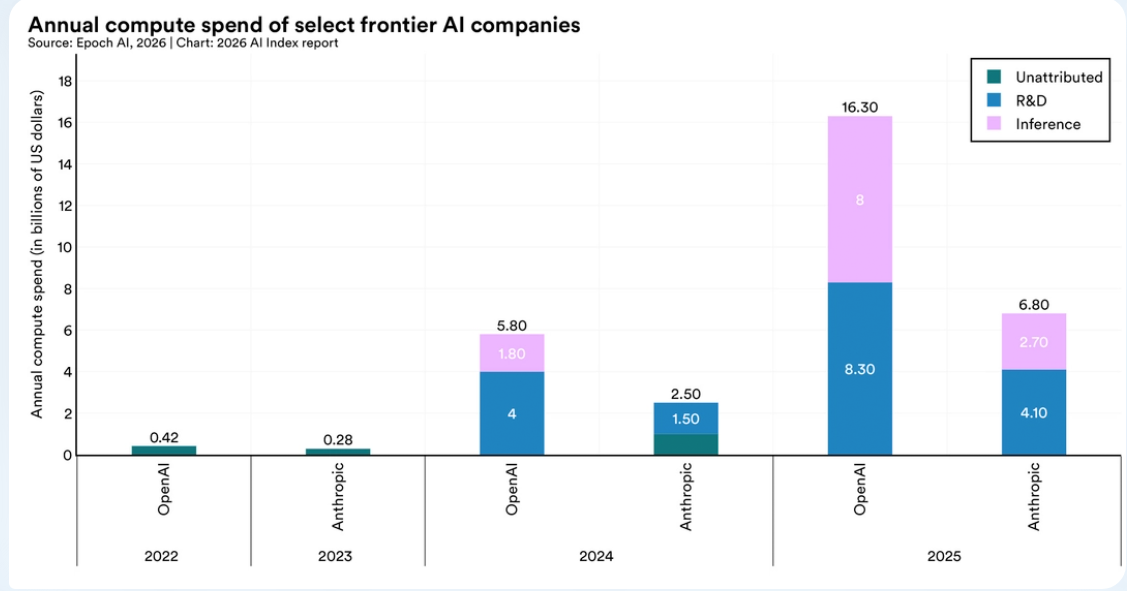
\includegraphics[scale=0.5]{AnnualAISpendings.png}
    \end{subfigure}
    
    \begin{subfigure}[H]{0.5\textwidth}
        \centering
        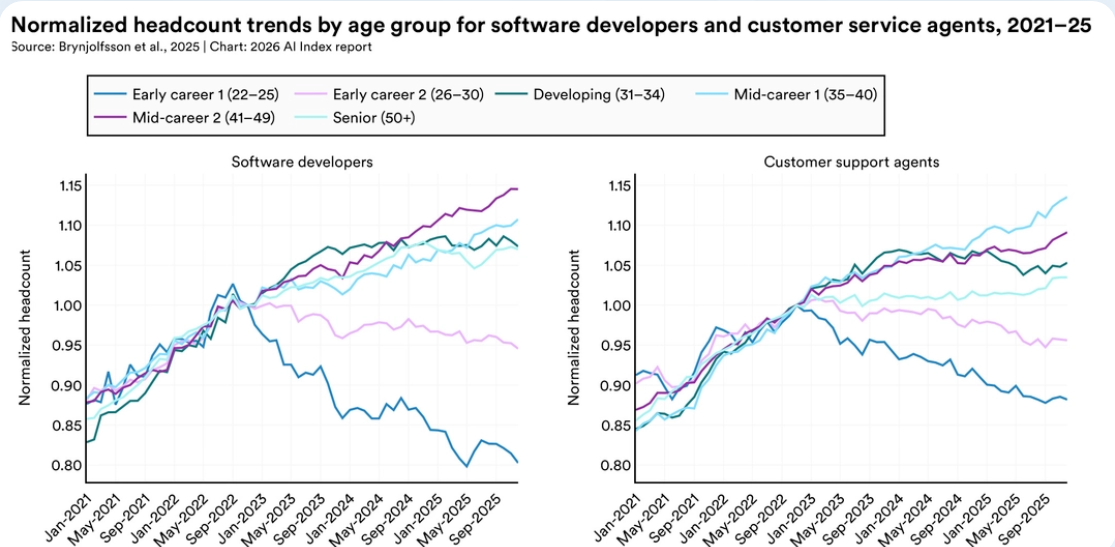
\includegraphics[scale=0.5]{SoftwareDevHeadCount.png}
    \end{subfigure}

\end{figure}


\end{document}